\chapter{背景介绍}
\section{ClickNP编程工具}
ClickNP是微软亚洲研究院开发的FPGA编程工具\cite{clicknp}。
\subsection{系统架构}
ClickNP基于Catapult Shell体系结构\cite{6853195}搭建。该体系结构包含PCIe、直接内存访问 (direct memory access, DMA)、
内存管理单元 (memory management unit, MMU)、以太网介质访问控制 (media access control, MAC)等
适用于多种应用场景的可服用逻辑,并将其抽象为定义好的接口。由ClickNP编写的FPGA程序生成的目标为Catapult功能。
由于ClickNP依赖的不同高级编程工具生成的目标接口不一致,因此在其下层有一个适配层,
将不同高级编程工具接口统一到Catapul Shell接口。

主机进程通过ClickNP库函数与FPGA程序通信,而库函数则依赖Catapult PCIe接口实现。
ClickNP库主要实现两个重要的功能:主机与FPGA之间的高速低延迟PCIe通道应用程序接口,
以及不同高级编程工具向FPGA模块传递参数并发送启动、停止、复位等信号的调用接口。

主机进程包括一个管理线程以及零个或多个工作线程。管理进程负责将程序镜像载入硬件、
启动工作进程、根据配置初始化FPGA和CPU中的ClickNP元件以及在运行时通过想各个元件发送信号来控制其行为。
在CPU的指派下,每个工作线程可以处理多个任务。

\subsection{程序设计}
\subsubsection{概念抽象}
ClickNP提供了模块化的编程模型,以元件为基本处理模块。每个元件包括以下属性:
\begin{description}
\item[本地状态]每个元件可定义一系列仅由自身访问的本地状态;
\item[输入输出端口]一个元件可以通过多个输入输出端口与其他元件通信;
\item[句柄函数]一个元件有三个句柄函数:初始化函数只在元件启动时执行一次;
处理函数在元件工作期间反复调用,处理输入的数据;信号函数类似于中断控制器,
在元件从主机进程收到信号时被调用,处理指令。
\end{description}

\begin{figure}[htbp]
\centering
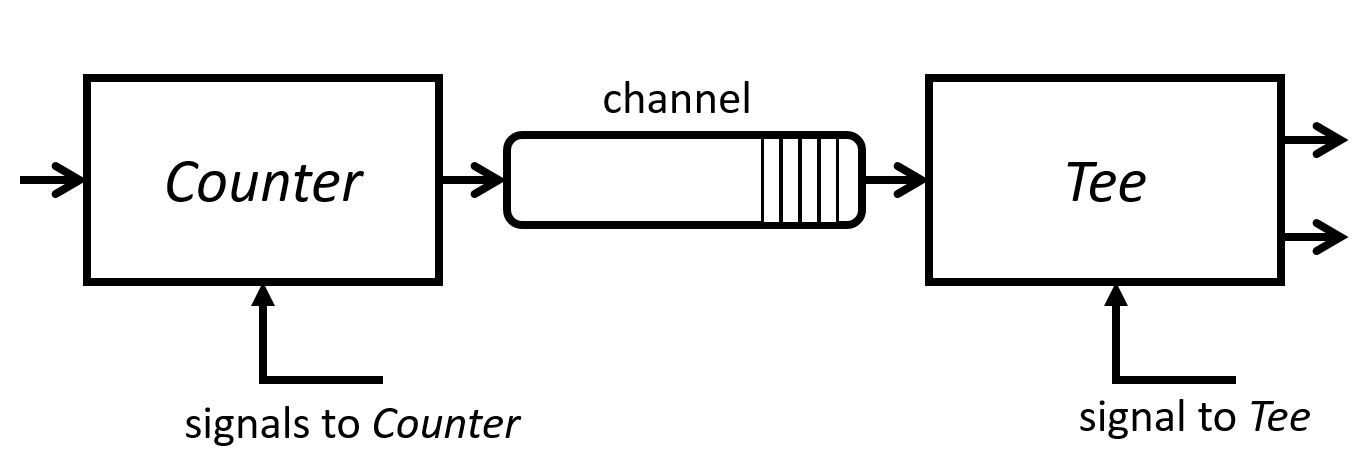
\includegraphics[width=4in]{channel}
\caption{连接两个元件的通道}\label{fig:channel}
\end{figure}

一个元件的输出端口可以用通道与另一个元件的输入端口连接。在ClickNP中,通道相当于一个先进先出的缓冲区,
从其一端写入,从另一端读取,如图~\ref{fig:channel} 所示。

\begin{figure}[htbp]
\centering

\includegraphics[width=4in]{flit}
\caption{帧结构}\label{fig:flit}
\end{figure}

\lstinputlisting[float, floatplacement=htbp, caption=帧成员定义, label=code:flitdef]{code/flit.cl}

每次通道读写操作的基本单位为帧,每个帧的大小固定为64字节,其中头部包含元数据,
数据载荷长32字节。其结构及成员定义如图~\ref{fig:flit}、代码~\ref{code:flitdef} 所示。

以完整包为代表的大段数据会被拆分为多个帧在元件之间传播。
其中第一帧的包开始位 (start of packet, \lstinline$sop$)置为真,
最后一帧的包结束位 (end of packet, \lstinline$eop$)置为真。
如果数据载荷小于32字节,那么最后一帧的留白 (padding, \lstinline$pad$)域指代载荷的尾部留白区段大小。
将大的包拆分为帧,不仅能够降低延迟,还有助于提升处理包数据的各级流水线之间并行化程度。

在定义完各个元件之后,通过ClickNP配置文件将元件连接为有向图,使其互连,形成总的计算系统。
代码~\ref{code:cfg} 是一个抓包器的配置文件,其开头部分将元件实例化,随后箭头表示其通道连接关系,
自左侧元件的输出端口指向右侧元件的输入端口,方括号中的数字代表端口号。
\begin{figure}[htbp]
\centering
\lstinputlisting[caption=ClickNP配置文件示例, label=code:cfg]{code/sample.cfg}
\note{@符号表示计数器\lstinline$cnt$从主机接收信号。
\lstinline$host$关键字代表将\lstinline$PktLogger$元件实例化为主机工作线程。
\lstinline$from_tor$和\lstinline$to_tor$分别为FPGA中网卡的输出和输入端口。}
\end{figure}

\subsubsection{编程语言}
ClickNP元件类似于面向对象语言中的对象,可以用C++这样的语言定义。
但现有的很多高级编程工具只支持C语言,而将高级语言转化为C语言的工作是乏味的,
因此我们采用的是针对定义元件的需要对C语言进行扩展这种途径。

\lstinputlisting[float, floatplacement=htbp, caption=包计数器元件定义, label=code:count]{code/Count.cl}
代码~\ref{code:count} 是一个包计数器元件的定义。\lstinline$.element$关键字定义元件名称;
尖括号内为输入输出端口数;\lstinline$.state$关键字定义本地状态\lstinline$count$计数器;
\lstinline$.init$关键字定义初始化函数,将\lstinline$count$的初值置零;
\lstinline$.handler$关键字定义处理函数,每当收到帧的\lstinline$sop$域为真时将计数器加一;
\lstinline$.signal$关键字定义信号函数,每当收到主机发来的任意信号帧时,
将当前包计数作为信号载荷发给主机。

ClickNP内建了一系列与端口进行数据交互的函数接口,如表~\ref{tab:operations} 所示。
\begin{table}[htbp]
\centering
\caption{ClickNP内建接口}\label{tab:operations}
\begin{tabular}{l l}
\toprule
\lstinline$uchar get_input_port()$         & 获取第一个有帧输入的端口号 \\
\midrule
\lstinline$bool test_input_port(uchar id)$ & 检查\lstinline$id$号端口有无帧输入 \\
\midrule
\lstinline$flit read_input_port(uchar id)$ & 自\lstinline$id$号端口读取帧 \\
\midrule
\lstinline$flit peek_input_port(uchar id)$ & 窥视\lstinline$id$号输入端口的帧 \\
\midrule
\lstinline$void set_output_port(uchar id,$ & 向\lstinline$id$号端口写入帧, \\
\lstinline$flit x)$                        & 在处理函数执行到返回时, \\
                                           & 该帧将被写入通道 \\
\midrule
\lstinline$ClSignal read_signal()$         & 自信号输入端口读取帧 \\
\midrule
\lstinline$void set_signal(ClSignal p)$    & 向信号输出端口写入帧 \\
\bottomrule
\end{tabular}
\end{table}

\subsubsection{编译工具链}
ClickNP工具链以ClickNP编译器为前端,以Visual Studio、GCC等C/C++编译器、
Altera OpenCL SDK、Xilinx Vidado HLS等高级编程工具为后端。
开发人员需要完成三部分工作:
\begin{enumerate}
\item 定义元件,每个元件实现一小部分简单的功能;
\item 编写配置文件,描述元件之间的连接关系,以组成完整的逻辑系统;
\item 设计主机管理进程,初始化各元件并在运行时根据用户输入控制元件行为。
\end{enumerate}

以上三部分源程序由ClickNP编译器翻译为主机程序和FPGA程序两部分中间代码。
前者可由普通的C/C++编译器编译为目标文件,
后者需要由商业化高级编程工具合成为FPGA目标文件。

\chapter{FPGA并行优化方法}
\section{元件间并行}
ClickNP的模块化架构自然地实现了不同元件之间的并行化,其工具链将元件实例映射到FPGA上的硬件区块,
不同区块间通过先进先出缓冲器连接,因而可以彼此独立地并行工作。
因此,ClickNP配置文件中的每个实例化元件均可视为具有专门功能的独立的核。
网络包以帧为单位在元件之间传播,各级元件可以流水化并行处理。
在单元件处理能力不足时,还可以通过增加元件数,实现数据级并行。
对于网络流量而言,流水线并行和数据并行均可用于加速其处理性能,
且在ClickNP平台上可以灵活地实现这些并行。

\section{元件内并行}
与逐条执行指令的CPU不同,FPGA通过硬件逻辑执行数据操作。
如果在一个处理函数中需要对单个数据进行多次操作,高级编程工具会将其转化为多级流水线操作。
每一时钟周期,将流水线推进一级,并移进新的数据,如图~\ref{fig:pipeline} 所示。

\begin{figure}[htbp]
\centering
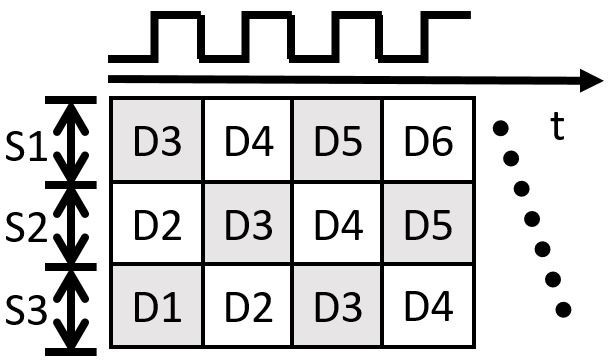
\includegraphics[width=4in]{pipeline}
\caption{多级流水线操作} \label{fig:pipeline}
\end{figure}

多级流水线操作可以使处理函数平均每个时钟周期处理完一单位数据,以实现吞吐率最大化。


\section{基于融合以太网络的RDMA协议}
基于融合以太网络的RDMA (RDMA over Converged Ethernet, RoCE) 协议允许设备间通过以太网络进行远程直接内存访问。
该协议有两个版本,分别称为RoCEv1和RoCEv2。其中RoCEv1将以太网协议作为其链路层协议,
因而允许在同一个以太网广播域下的任意两台主机间进行通信\cite{a16}。
RoCEv2则基于用户数据报协议 (user datagram protocol, UDP),因而可以经过路由\cite{a17, considerations, storage}。

\subsection{术语解释}
\begin{description}
\item[通信管理器 (communication manager, CM)]支持通信管理协议机制的软件或硬件,或软硬件结合体。
\item[可靠连接 (reliable connection, RC)]由发送和接收一对互相关联的工作队列实现的工作机制,
其中一个工作队列发出的包一定被另一个工作队列接收。
\item[不可靠报文 (unreliable datagram)]将发送工作队列关联至接收工作队列的工作机制,
其中发送队列发出的包只可能被接收队列而非其他队列接收。\cite{volume1}
\end{description}

\subsection{工作原理}
\begin{figure}[htbp]
\centering
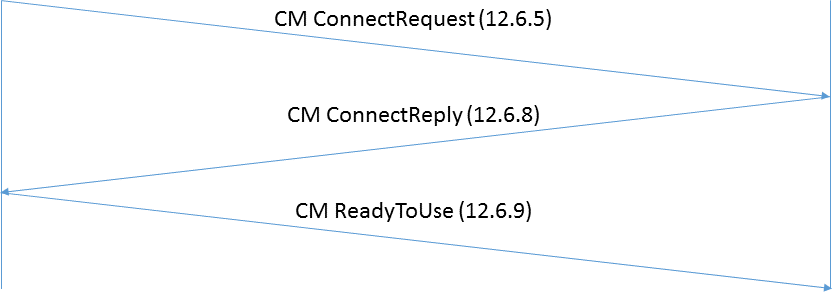
\includegraphics[width=4in]{rocereq}
\caption{建立RoCE连接}\label{fig:rocereq}
\end{figure}

\begin{figure}[htbp]
\centering
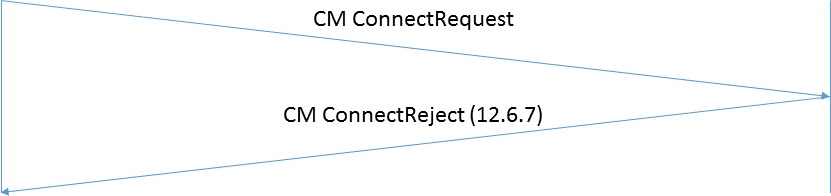
\includegraphics[width=4in]{rocerej}
\caption{建立RoCE连接被拒绝}\label{fig:rocerej}
\end{figure}

\begin{figure}[htbp]
\centering
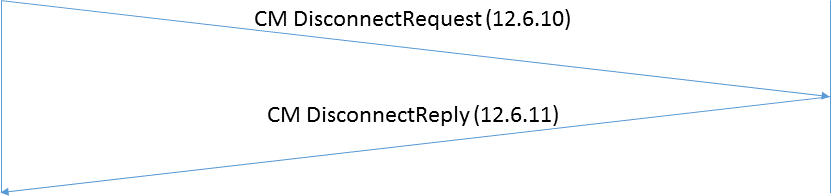
\includegraphics[width=4in]{rocedreq}
\caption{断开RoCE连接}\label{fig:rocedreq}
\end{figure}

\begin{figure}[htbp]
\centering
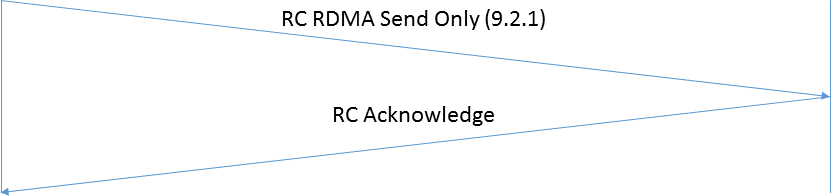
\includegraphics[width=4in]{rocewriteonly}
\caption{单RoCE包写操作}\label{fig:rocewriteonly}
\note{在数据载荷不多于1024字节时的写请求只包含单包,数据发送请求的工作过程与之类似。}
\end{figure}

\begin{figure}[htbp]
\centering
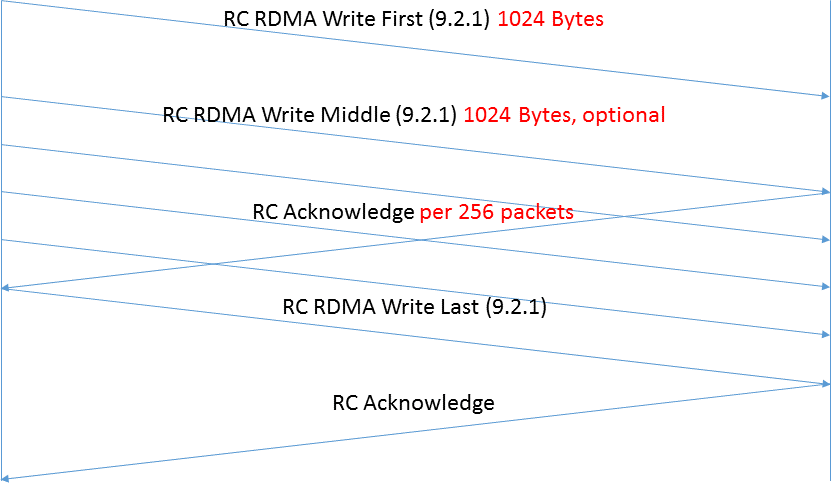
\includegraphics[width=4in]{rocewritemany}
\caption{多RoCE包写操作}\label{fig:rocewritemany}
\note{对于超过1024字节的数据载荷,先后发送Write First、Write Middle (如有)、Write Last三种包。
自Write First起,接收端每收到256个包反馈一个确认包,也对最后一个包进行反馈,
数据发送请求的工作过程与之类似。}
\end{figure}

\begin{figure}[htbp]
\centering
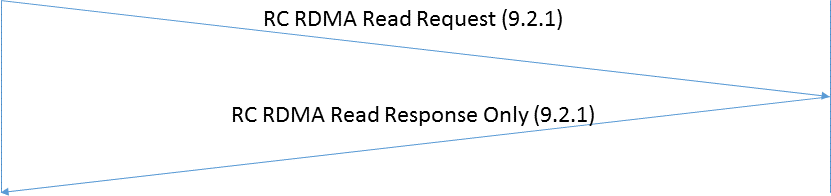
\includegraphics[width=4in]{rocereadonly}
\caption{单RoCE包读操作}\label{fig:rocereadonly}
\note{在数据载荷不多于1024字节时读响应只包含单包}
\end{figure}

\begin{figure}[htbp]
\centering
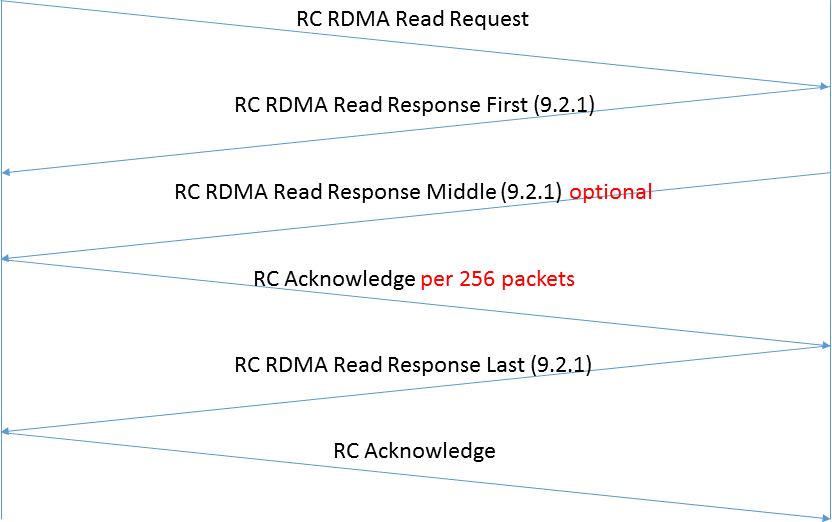
\includegraphics[width=4in]{rocereadmany}
\caption{多RoCE包读操作}\label{fig:rocereadmany}
\note{对于超过1024字节的数据载荷,先后发送Read Response First、Read Response Middle (如有)、
Read Response Last三种包。自Read Response First起,接收端每收到256个包反馈一个确认包,
也对最后一个包进行反馈。}
\end{figure}

用户可通过RoCE协议发起读数据、写数据、发送数据三种请求。
其工作过程如图~\ref{fig:rocereq}、图~\ref{fig:rocerej}、图~\ref{fig:rocedreq}、
图~\ref{fig:rocewriteonly}、图~\ref{fig:rocewritemany}、图~\ref{fig:rocereadonly}所示。

面对网络中可能出现的丢包情况,RoCE协议具有与TCP/IP类似的重传策略:
对每个消息赋予一个包序列号。如果接收端收到的包序列号不连续,则反馈缺失消息,
并提供缺失的第一个包序列号。发送端从该序列号对应的包开始重传,如图~\ref{fig:rocewritenak} 所示。
\begin{figure}[htbp]
\centering
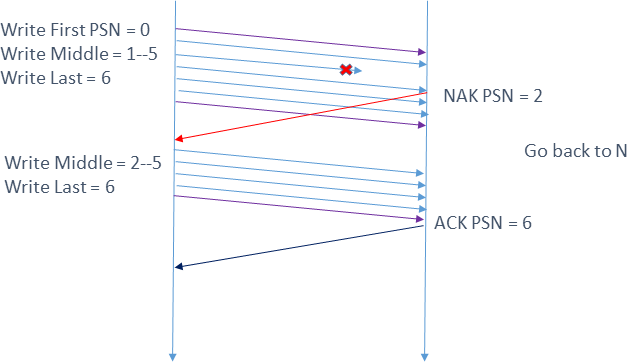
\includegraphics[width=4in]{rocewritenak}
\caption{RoCE重传策略}\label{fig:rocewritenak}
\end{figure}
